
%{{第四十六回}}{第四十六回}}

\chapter{尴尬人难免尴尬事 鸳鸯女誓绝鸳鸯偶}\label{part0050_split_000.htmlux5cux23calibre_pb_0}

{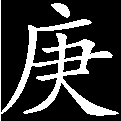
\includegraphics[width=3mm]{../Images/00004}此回亦有本而笔,非泛泛之笔也。}

{只看他题纲用``尴尬''二字于邢夫人,可知包藏含蓄文字之中,莫能量也。}

{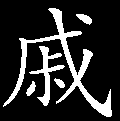
\includegraphics[width=3mm]{../Images/00005}裹脚与缠头,欲觅终身伴。顾影自为怜,静住深深院。 好事不称心,恶语将人慢。誓死守香闺,远却杨花片。}

话说林黛玉直到四更将阑,方渐渐的睡去,暂且无话。

如今且说凤姐儿因见邢夫人叫他,不知何事,忙另穿戴了一番,坐车过来。邢夫人将房内人遣出,悄向凤姐儿道:``叫你来不为别事,有一件为难的事,老爷托我,我不得主意,先和你商议。老爷因看上了老太太的鸳鸯,要他在房里,叫我和老太太讨去。我想这倒平常有的事,只是怕老太太不给,你可有法子?''凤姐儿听了,忙道:``依我说,竟别碰这个钉子去。老太太离了鸳鸯,饭也吃不下去的,那里就舍得了?况且平日说起闲话来,老太太常说,老爷如今上了年纪,作什么左一个小老婆右一个小老婆放在屋里,没的耽误了人家。放着身子不保养,官儿也不好生作去,成日家和小老婆喝酒。太太听这话,很喜欢老爷呢?这会子回避还恐回避不及,倒拿草棍儿戳老虎的鼻子眼儿去了!太太别恼,我是不敢去的。明放着不中用,而且反招出没意思来。老爷如今上了年纪,行事不妥,太太该劝才是。比不得年轻,作这些事无碍。如今兄弟、侄儿、儿子、孙子一大群,还这么闹起来,怎样见人呢?''邢夫人冷笑道:``大家子三房四妾的也多,偏咱们就使不得?我劝了也未必依。就是老太太心爱的丫头,这么胡子苍白了又作了官的一个大儿子,要了作房里人,也未必好驳回的。我叫了你来,不过商议商议,你先派上了一篇不是。也有叫你去的理?自然是我说去。你倒说我不劝,你还不知道那性子的,劝不成,先和我恼了。''

凤姐儿知道邢夫人禀性愚犟,只知承顺贾赦以自保,次则婪聚财货为自得,家下一应大小事务,俱由贾赦摆布。凡出入银钱事务,一经他手,便克啬异常,以贾赦浪费为名,``须得我就中俭省,方可偿补'',儿女奴仆,一人不靠,一言不听的。如今又听邢夫人如此的话,便知他又弄左性,劝了不中用,连忙陪笑说道:``太太这话说的极是。我能活了多大,知道什么轻重?想来父母跟前,别说一个丫头,就是那么大的活宝贝,不给老爷给谁?背地里的话那里信得?我竟是个呆子。琏二爷或有日得了不是,老爷太太恨的那样,恨不得立刻拿来一下子打死;及至见了面,也罢了,依旧拿着老爷太太心爱的东西赏他。如今老太太待老爷,自然也是那样了。依我说,老太太今儿喜欢,要讨今儿就讨去。我先过去哄着老太太发笑,等太太过去了,我搭讪着走开,把屋子里的人我也带开,太太好和老太太说的。给了更好,不给也没妨碍,众人也不知道。''邢夫人见他这般说,便又喜欢起来,又告诉他道:``我的主意先不和老太太要。老太太要说不给,这事便死了。我心里想着先悄悄的和鸳鸯说。他虽害臊,我细细的告诉了他,他自然不言语,就妥了。那时再和老太太说,老太太虽不依,搁不住他愿意,常言`人去不中留',自然这就妥了。''凤儿姐笑道:``到底是太太有智谋,这是千妥万妥的。别说是鸳鸯,凭他是谁,那一个不想巴高望上,不想出头的?这半个主子不做,倒愿意做个丫头,将来配个小子就完了。''邢夫人笑道:``正是这个话了。别说鸳鸯,就是那些执事的大丫头,谁不愿意这样呢。你先过去,别露一点风声,我吃了晚饭就过来。''

凤姐儿暗想:``鸳鸯素习是个可恶的,虽如此说,保不严他就愿意。我先过去了,太太后过去,若他依了便没话说;倘或不依,太太是多疑的人,只怕就疑我走了风声,使他拿腔作势的。那时太太又见了应了我的话,羞恼变成怒,拿我出起气来,倒没意思。不如同着一齐过去了,他依也罢,不依也罢,就疑不到我身上了。''想毕,因笑道:``方才临来,舅母那边送了两笼子鹌鹑,我吩咐他们炸了,原要赶太太晚饭上送过来的。我才进大门时,见小子们抬车,说太太的车拔了缝,拿去收拾去了。不如这会子坐了我的车一齐过去倒好。''邢夫人听了,便命人来换衣服。凤姐忙着伏侍了一回,娘儿两个坐车过来。凤姐儿又说道:``太太过老太太那里去,我若跟了去,老太太若问起我过去作什么的,倒不好。不如太太先去,我脱了衣裳再来。''

邢夫人听了有理,便自往贾母处,和贾母说了一回闲话,便出来假托往王夫人房里去,从后门出去,打鸳鸯的卧房前过。只见鸳鸯正然坐在那里做针线,见了邢夫人,忙站起来。邢夫人笑道:``做什么呢?我瞧瞧,你扎的花儿越发好了。''一面说,一面便接他手内的针线瞧了一瞧,只管赞好。放下针线,又浑身打量。只见他穿着半新的藕合色的绫袄,青缎掐牙背心,下面水绿裙子。蜂腰削背,鸭蛋脸面,乌油头发,高高的鼻子,两边腮上微微的几点雀斑。鸳鸯见这般看他,自己倒不好意思起来,心里便觉诧异,因笑问道:``太太,这会子不早不晚的,过来做什么?''邢夫人使个眼色儿,跟的人退出。邢夫人便坐下,拉着鸳鸯的手笑道:``我特来给你道喜来了。''鸳鸯听了,心中已猜着三分,不觉红了脸,低了头不发一言。听邢夫人道:``你知道你老爷跟前竟没有个可靠的人,{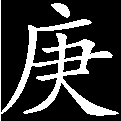
\includegraphics[width=3mm]{../Images/00004}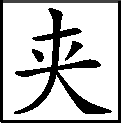
\includegraphics[width=3mm]{../Images/00012}\footnotesize \kaishu 说得得体。我正想开口一句不知如何说,如此则妙极是极,如闻如见。}心里再要买一个,又怕那些人牙子家出来的不干不净,也不知道毛病儿,买了来家,三日两日,又要肏鬼吊猴的。因满府里要挑一个家生女儿收了,又没个好的:不是模样儿不好,就是性子不好,有了这个好处,没了那个好处。因此冷眼选了半年,这些女孩子里头,就只你是个尖儿,模样儿,行事作人,温柔可靠,一概是齐全的。意思要和老太太讨了你去,收在屋里。你比不得外头新买的,你这一进去了,进门就开了脸,就封你姨娘,又体面,又尊贵。你又是个要强的人,俗语说的,`金子终得金子换',谁知竟被老爷看重了你。如今这一来,你可遂了素日志大心高的愿了,也堵一堵那些嫌你的人的嘴。跟了我回老太太去!''说着拉了他的手就要走。鸳鸯红了脸,夺手不行。邢夫人知他害臊,因又说道:``这有什么臊处?你又不用说话,只跟着我就是了。''鸳鸯只低了头不动身。邢夫人见他这般,便又说道:``难道你不愿意不成?若果然不愿意,可真是个傻丫头了。放着主子奶奶不作,倒愿意作丫头!三年二年,不过配上个小子,还是奴才。你跟了我们去,你知道我的性子又好,又不是那不容人的人。老爷待你们又好。过一年半载,生下个一男半女,你就和我并肩了。家里的人你要使唤谁,谁还不动?现成主子不做去,错过这个机会,后悔就迟了。''鸳鸯只管低了头,仍是不语。邢夫人又道:``你这么个响快人,怎么又这样积粘起来?有什么不称心之处,只管说与我,我管你遂心如意就是了。''鸳鸯仍不语。邢夫人又笑道:``想必你有老子娘,你自己不肯说话,怕臊。你等他们问你,这也是理。让我问他们去,叫他们来问你,有话只管告诉他们。''说毕,便往凤姐儿房中来。

凤姐儿早换了衣服,因房内无人,便将此话告诉了平儿。平儿也摇头笑道:``据我看,此事未必妥。平常我们背着人说起话来,听他那主意,未必是肯的。也只说着瞧罢了。''凤姐儿道:``太太必来这屋里商议。依了还可,若不依,白讨个臊,当着你们,岂不脸上不好看。你说给他们炸鹌鹑,再有什么配几样,预备吃饭。你且别处逛逛去,估量着去了再来。''平儿听说,照样传给婆子们,便逍遥自在的往园子里来。

这里鸳鸯见邢夫人去了,必在凤姐儿房里商议去了,必定有人来问他的,不如躲了这里,{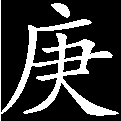
\includegraphics[width=3mm]{../Images/00004}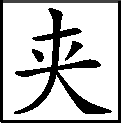
\includegraphics[width=3mm]{../Images/00012}\footnotesize \kaishu 终不免女儿气,不知躲在那里方无人来罗唣,写得可怜可爱。}因找了琥珀说道:``老太太要问我,只说我病了,没吃早饭,往园子里逛逛就来。''琥珀答应了。鸳鸯也往园子里来,各处游玩,不想正遇见平儿。平儿因见无人,便笑道:``新姨娘来了!''鸳鸯听了,便红了脸,说道:``怪道你们串通一气来算计我!等着我和你主子闹去就是了。''平儿听了,自悔失言,便拉他到枫树底下,{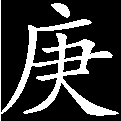
\includegraphics[width=3mm]{../Images/00004}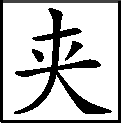
\includegraphics[width=3mm]{../Images/00012}\footnotesize \kaishu 随笔带出妙景。正愁园中草木黄落,不想看此一句,便恍如置身于千霞万锦、绛雪红霜之中矣。}坐在一块石上,越性把方才凤姐过去回来所有的形景言词、始末原由告诉与他。鸳鸯红了脸,向平儿冷笑道:``这是咱们好,比如袭人、琥珀、素云、紫鹃、彩霞、玉钏儿、麝月、翠墨,跟了史姑娘去的翠缕,死了的可人和金钏,去了的茜雪,{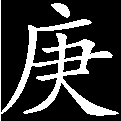
\includegraphics[width=3mm]{../Images/00004}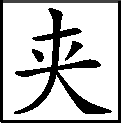
\includegraphics[width=3mm]{../Images/00012}\footnotesize \kaishu 余按此一算,亦是十二钗,真镜中花,水中月,云中豹,林中之鸟,穴中之鼠,无数可考,无人可指,有迹可追,有形可据,九曲八折,远响近影,迷离烟灼,纵横隐现,千奇百怪,眩目移神,现千手千眼大游戏法也。脂砚斋。}连上你我,这十来个人,从小儿什么话儿不说?什么事儿不作?这如今因都大了,各自干各自的去了,{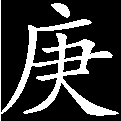
\includegraphics[width=3mm]{../Images/00004}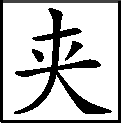
\includegraphics[width=3mm]{../Images/00012}\footnotesize \kaishu 此语已可伤,犹未``各自干各自去'',后日更有各自之处也,知之乎!}然我心里仍是照旧,有话有事,并不瞒你们。这话我且放在你心里,且别和二奶奶说:别说大老爷要我做小老婆,就是太太这会子死了,他三媒六聘的娶我去作大老婆,我也不能去。''

平儿方欲笑答,只听山石背后哈哈的笑道:``好个没脸的丫头,亏你不怕牙碜。''二人听了不免吃了一惊,忙起身向山石背后找寻,不是别个,却是袭人笑着走了出来问:``什么事情?告诉我。''说着,三人坐在石上,平儿又把方才的话说与袭人听。袭人道:``真真这话论理不该我们说,这个大老爷太好色了,略平头正脸的,他就不放手了。''平儿道:``你既不愿意,我教你个法子,不用费事就完了。''鸳鸯道:``什么法子?你说来我听。''平儿笑道:``你只和老太太说,就说已经给了琏二爷了,大老爷就不好要了。''鸳鸯啐道:``什么东西!你还说呢!前儿你主子不是这么混说的?谁知应到今儿了!''袭人笑道:``他们两个都不愿意,我就和老太太说,叫老太太说把你已经许了宝玉了,大老爷也就死了心了。''鸳鸯又是气,又是臊,又是急,因骂道:``两个蹄子不得好死的!人家有为难的事,拿着你们当正经人,告诉你们与我排解排解,你们倒替换着取笑儿。你们自为都有了结果了,将来都是做姨娘的。据我看,天下的事未必都遂心如意。你们且收着些儿,别忒乐过了头儿!''二人见他急了,忙陪笑央告道:``好姐姐,别多心,咱们从小儿都是亲姊妹一般,不过无人处偶然取个笑儿。你的主意告诉我们知道,也好放心。''鸳鸯道:``什么主意!我只不去就完了。''平儿摇头道:``你不去未必得干休。大老爷的性子你是知道的。虽然你是老太太房里的人,此刻不敢把你怎么样,将来难道你跟老太太一辈子不成?也要出去的。那时落了他的手,倒不好了。''鸳鸯冷笑道:``老太太在一日,我一日不离这里;若是老太太归西去了,他横竖还有三年的孝呢,没个娘才死了他先纳小老婆的!等过三年,知道又是怎么个光景,那时再说。纵到了至急为难,我剪了头发作姑子去;不然,还有一死。一辈子不嫁男人,又怎么样?乐得干净呢!''平儿袭人笑道:``真这蹄子没了脸,越发信口儿都说出来了。''鸳鸯道:``事到如此,臊一会怎么样!你们不信,慢慢的看着就是了。太太才说了,找我老子娘去。我看他南京找去!''平儿道:``你的父母都在南京看房子,没上来,终久也寻的着。现在还有你哥哥嫂子在这里。可惜你是这里的家生女儿,不如我们两个人是单在这里。''鸳鸯道:``家生女儿怎么样?`牛不吃水强按头'?我不愿意,难道杀我的老子娘不成?''

正说着,只见他嫂子从那边走来。袭人道:``当时找不着你的爹娘,一定和你嫂子说了。''鸳鸯道:``这个娼妇专管是个`九国贩骆驼的',听了这话,他有个不奉承去的!''说话之间,已来到跟前。他嫂子笑道:``那里没找到,姑娘跑了这里来!你跟了我来,我和你说话。''平儿袭人都忙让坐。他嫂子说:``姑娘们请坐,我找我们姑娘说句话。''袭人平儿都装不知道,笑道:``什么话这样忙?我们这里猜谜儿赢手批子打呢,等猜了这个再去。''鸳鸯道:``什么话?你说罢。''他嫂子笑道:``你跟我来,到那里我告诉你,横竖有好话儿。''鸳鸯道:``可是大太太和你说的那话?''他嫂子笑道:``姑娘既知道,还奈何我!快来,我细细的告诉你可是天大的喜事。''鸳鸯听说,立起身来,照他嫂子脸上下死劲啐了一口,指着他骂道:``你快夹着屄嘴离了这里,好多着呢!什么`好话'!宋徽宗的鹰,赵子昂的马,都是好画儿。什么`喜事'!状元痘儿灌的浆儿又满是喜事。怪道成日家羡慕人家女儿作了小老婆了,一家子都仗着他横行霸道的,一家子都成了小老婆了!看的眼热了,也把我送在火坑里去。我若得脸呢,你们外头横行霸道,自己就封自己是舅爷了。我若不得脸败了时,你们把忘八脖子一缩,生死由我。''一面说,一面哭,平儿袭人拦着劝。

他嫂子脸上下不来,因说道:``愿意不愿意,你也好说,不犯着牵三挂四的。俗语说,`当着矮人,别说短话'。姑奶奶骂我,我不敢还言;这二位姑娘并没惹着你,小老婆长小老婆短,大家脸上怎么过得去?''袭人平儿忙道:``你倒别这么说,他也并不是说我们,你倒别牵三挂四的。你听见那位太太、太爷们封我们做小老婆?况且我们两个也没有爹娘、哥哥兄弟在这门子里仗着我们横行霸道的。他骂的人自有他骂的,我们犯不着多心。''鸳鸯道:``他见我骂了他,他臊了,没的盖脸,又拿话挑唆你们两个,幸亏你们两个明白。原是我急了,也没分别出来,他就挑出这个空儿来。''他嫂子自觉没趣,赌气去了。鸳鸯气得还骂,平儿袭人劝他一回,方才罢了。

平儿因问袭人道:``你在那里藏着做甚么的?我们竟没看见你。''袭人道:``我因为往四姑娘房里瞧我们宝二爷去的,谁知迟了一步,说是来家里来了。我疑惑怎么不遇见呢,想要往林姑娘家里找去,又遇见他的人说也没去。我这里正疑惑是出园子去了,可巧你从那里来了,我一闪,你也没看见。后来他又来了。我从这树后头走到山子石后,我却见你两个说话来了,谁知你们四个眼睛没见我。''

一语未了,又听身后笑道:``四个眼睛没见你?你们六个眼睛竟没见我!''三人唬了一跳,回身一看,不是别个,正是宝玉走来。{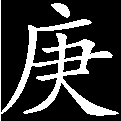
\includegraphics[width=3mm]{../Images/00004}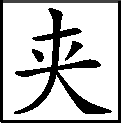
\includegraphics[width=3mm]{../Images/00012}\footnotesize \kaishu 通部情案,皆必从石兄挂号,然各有各稿,穿插神妙。}袭人先笑道:``叫我好找,你那里来?''宝玉笑道:``我从四妹妹那里出来,迎头看见你来了,我就知道是找我去的,我就藏了起来哄你。看你低着头过去了,进了院子就出来了,逢人就问。我在那里好笑,只等你到了跟前唬你一跳的,后来见你也藏藏躲躲的,我就知道也是要哄人了。我探头往前看了一看,却是他两个,所以我就绕到你身后。你出去,我就躲在你躲的那里了。''平儿笑道:``咱们再往后找找去,只怕还找出两个人来也未可知。''宝玉笑道:``这可再没了。''鸳鸯已知话俱被宝玉听了,只伏在石头上装睡。宝玉推他笑道:``这石头上冷,咱们回房里去睡,岂不好?''说着拉起鸳鸯来,又忙让平儿来家坐吃茶。平儿和袭人都劝鸳鸯走,鸳鸯方立起身来,四人竟往怡红院来。宝玉将方才的话俱已听见,心中自然不快,只默默的歪在床上,任他三人在外间说笑。

外边邢夫人因问凤姐儿鸳鸯的父母,凤姐因回说:``他爹的名字叫金彩,{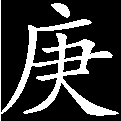
\includegraphics[width=3mm]{../Images/00004}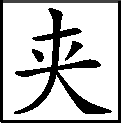
\includegraphics[width=3mm]{../Images/00012}\footnotesize \kaishu 姓金名彩,由``鸳鸯''二字化出,因文而生文也。}两口子都在南京看房子,从不大上京。他哥哥金文翔,{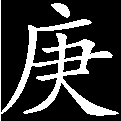
\includegraphics[width=3mm]{../Images/00004}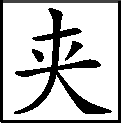
\includegraphics[width=3mm]{../Images/00012}\footnotesize \kaishu 更妙!}现在是老太太那边的买办。他嫂子也是老太太那边浆洗的头儿。''{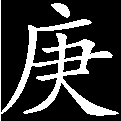
\includegraphics[width=3mm]{../Images/00004}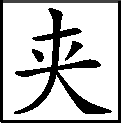
\includegraphics[width=3mm]{../Images/00012}\footnotesize \kaishu 只鸳鸯一家,写的荣府中人各有各职,如目已睹。}邢夫人便令人叫了他嫂子金文翔媳妇来,细细说与他。金家媳妇自是喜欢,兴兴头头找鸳鸯,只望一说必妥,不想被鸳鸯抢白一顿,又被袭人平儿说了几句,羞恼回来,便对邢夫人说:``不中用,他倒骂了我一场。''因凤姐儿在旁,不敢提平儿,只说:``袭人也帮着他抢白我,也说了许多不知好歹的话,回不得主子的。太太和老爷商议再买罢。谅那小蹄子也没有这么大福,我们也没有这么大造化。''邢夫人听了,因说道:``又与袭人什么相干?他们如何知道的?''又问:``还有谁在跟前?''金家的道:``还有平姑娘。''凤姐儿忙道:``你不该拿嘴巴子打他回来?我一出了门,他就逛去了;回家来连一个影儿也摸不着他!他必定也帮着说什么呢!''金家的道:``平姑娘没在跟前,远远的看着倒像是他,可也不真切,不过是我白忖度。''凤姐便命人去:``快打了他来,告诉他我来家了,太太也在这里,请他来帮个忙儿。''丰儿忙上来回道:``林姑娘打发了人下请字请了三四次,他才去了。奶奶一进门我就叫他去的。林姑娘说:`告诉你奶奶,我烦他有事呢。'''凤姐儿听了方罢,故意的还说:``天天烦他,有些什么事!''

邢夫人无计,吃了饭回家,晚间告诉了贾赦。贾赦想了一想,即刻叫贾琏来说:``南京的房子还有人看着,不止一家,即刻叫上金彩来。''贾琏回道:``上次南京信来,金彩已经得了痰迷心窍,那边连棺材银子都赏了,不知如今是死是活,便是活着,人事不知,叫来也无用。他老婆子又是个聋子。''贾赦听了,喝了一声,又骂:``下流囚攮的,偏你这么知道,还不离了我这里!''唬得贾琏退出,一时又叫传金文翔。贾琏在外书房伺候着,又不敢家去,又不敢见他父亲,只得听着。一时金文翔来了,小幺儿们直带入二门里去,隔了五六顿饭的工夫才出来去了。贾琏暂且不敢打听,隔了一会,又打听贾赦睡了,方才过来。至晚间凤姐儿告诉他,方才明白。

鸳鸯一夜没睡,至次日,他哥哥回贾母接他家去逛逛,贾母允了,命他出去。鸳鸯意欲不去,只怕贾母疑心,只得勉强出来。他哥哥只得将贾赦的话说与他,又许他怎么体面,又怎么当家作姨娘。鸳鸯只咬定牙不愿意。他哥哥无法,少不得去回覆了贾赦。贾赦怒起来,因说道:``我这话告诉你,叫你女人向他说去,就说我的话:`自古嫦娥爱少年',他必定嫌我老了,大约他恋着少爷们,多半是看上了宝玉,只怕也有贾琏。果有此心,叫他早早歇了心,我要他不来,此后谁还敢收?此是一件。第二件,想着老太太疼他,将来自然往外聘作正头夫妻去。叫他细想,凭他嫁到谁家去,也难出我的手心。除非他死了,或是终身不嫁男人,我就伏了他!若不然时,叫他趁早回心转意,有多少好处。''贾赦说一句,金文翔应一声``是''。贾赦道:``你别哄我,我明儿还打发你太太过去问鸳鸯,你们说了,他不依,便没你们的不是。若问他,他再依了,仔细你的脑袋!''

金文翔忙应了又应,退出回家,也不等得告诉他女人转说,竟自已对面说了这话。把个鸳鸯气的无话可回,想了一想,便说道:``便愿意去,也须得你们带了我回声老太太去。''他哥嫂听了,只当回想过来,都喜之不胜。他嫂子即刻带了他上来见贾母。

可巧王夫人、薛姨妈、李纨、凤姐儿、宝钗等姊妹并外头的几个执事有头脸的媳妇,都在贾母跟前凑趣儿呢。鸳鸯喜之不尽,拉了他嫂子,到贾母跟前跪下,一行哭,一行说,把邢夫人怎么来说,园子里他嫂子又如何说,今儿他哥哥又如何说,``因为不依,方才大老爷越性说我恋着宝玉,不然要等着往外聘,我到天上,这一辈子也跳不出他的手心去,终久要报仇。我是横了心的,当着众人在这里,我这一辈子莫说是`宝玉',便是`宝金'`宝银'`宝天王'`宝皇帝',横竖不嫁人就完了!就是老太太逼着我,我一刀子抹死了,也不能从命!若有造化,我死在老太太之先;若没造化,该讨吃的命,伏侍老太太归了西,我也不跟着我老子娘哥哥去,我或是寻死,或是剪了头发当尼姑去!若说我不是真心,暂且拿话来支吾,日后再图别的,天地鬼神,日头月亮照着嗓子,从嗓子里头长疔烂了出来,烂化成酱在这里!''

原来他一进来时,便袖了一把剪子,一面说着,一面左手打开头发,右手便铰。众婆娘丫鬟忙来拉住,已剪下半绺来了。众人看时,幸而他的头发极多,铰的不透,连忙替他挽上。贾母听了,气的浑身乱战,口内只说:``我通共剩了这么一个可靠的人,他们还要来算计!''因见王夫人在旁,便向王夫人道:``你们原来都是哄我的!外头孝敬,暗地里盘算我。有好东西也来要,有好人也要,剩了这么个毛丫头,见我待他好了,你们自然气不过,弄开了他,好摆弄我!''王夫人忙站起来,不敢还一言。{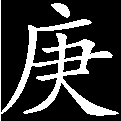
\includegraphics[width=3mm]{../Images/00004}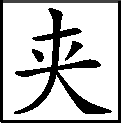
\includegraphics[width=3mm]{../Images/00012}\footnotesize \kaishu 千奇百怪,王夫人亦有罪乎?老人家迁怒之言必应如此。}薛姨妈见连王夫人怪上,反不好劝的了。李纨一听见鸳鸯的话,早带了姊妹们出去。

探春有心的人,想王夫人虽有委曲,如何敢辩;薛姨妈也是亲姊妹,自然也不好辩的;宝钗也不便为姨母辩;李纨、凤姐、宝玉一概不敢辩;这正用着女孩儿之时,迎春老实,惜春小,因此窗外听了一听,便走进来陪笑向贾母道:``这事与太太什么相干?老太太想一想,也有大伯子要收屋里的人,小婶子如何知道?便知道,也推不知道。''犹未说完,贾母笑道:``可是我老糊涂了!姨太太别笑话我。你这个姐姐他极孝顺我,不像我那大太太一味怕老爷,婆婆跟前不过应景儿。可是委屈了他。''薛姨妈只答应``是'',又说:``老太太偏心,多疼小儿子媳妇,也是有的。''贾母道:``不偏心!''因又说道:``宝玉,我错怪了你娘,你怎么也不提我,看着你娘受委屈?''宝玉笑道:``我偏着娘说大爷大娘不成?通共一个不是,我娘在这里不认,却推谁去?我倒要认是我的不是,老太太又不信。''贾母笑道:``这也有理。你快给你娘跪下,你说太太别委屈了,老太太有年纪了,看着宝玉罢。''宝玉听了,忙走过去,便跪下要说;王夫人忙笑着拉他起来,说:``快起来,快起来,断乎使不得。终不成你替老太太给我赔不是不成?''宝玉听说,忙站起来。{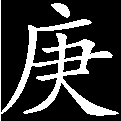
\includegraphics[width=3mm]{../Images/00004}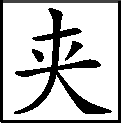
\includegraphics[width=3mm]{../Images/00012}\footnotesize \kaishu 宝玉亦有罪了。}

贾母又笑道:``凤姐儿也不提我。''{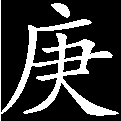
\includegraphics[width=3mm]{../Images/00004}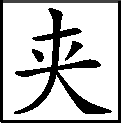
\includegraphics[width=3mm]{../Images/00012}\footnotesize \kaishu 阿凤也有了罪。◇奇奇怪怪之文,所谓《石头记》不是作出来的。}凤姐儿笑道:``我倒不派老太太的不是,老太太倒寻上我了?''贾母听了,与众人都笑道:``这可奇了!倒要听听这不是。''凤姐儿道:``谁教老太太会调理人,调理的水葱儿似的,怎么怨得人要?我幸亏是孙子媳妇,若是孙子,我早要了,还等到这会子呢。''贾母笑道:``这倒是我的不是了?''凤姐儿笑道:``自然是老太太的不是了。''贾母笑道:``这样,我也不要了,你带了去罢!''凤姐儿道:``等着修了这辈子,来生托生男人,我再要罢。''贾母笑道:``你带了去,给琏儿放在屋里,看你那没脸的公公还要不要了!''凤姐儿道:``琏儿不配,就只配我和平儿这一对烧糊了的卷子和他混罢。''说的众人都笑起来了。

丫鬟回说:``大太太来了。''王夫人忙迎了出去。要知端的------

{  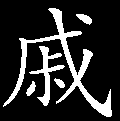
\includegraphics[width=3mm]{../Images/00005}总评:鸳鸯女从热闹中别具一副肠胃,``不轻许人''一事,是宦途中药石仙方。}

